\chapter{Services Computing - REST}
\section{Web Services Evolution}
Initially only HTML and HTTP, so services were limited to providing web pages.
\\With SOAP the services are strongly characterized and precisely described. They could even be "compiled". However, services are complex and difficult to describe and understand.
\\In REST, we \textbf{go back to the principles of HTTP} by eliminating redundancies and assigning semantics to verbs (GET, POST, PUT...) and URIs.
\begin{center}
    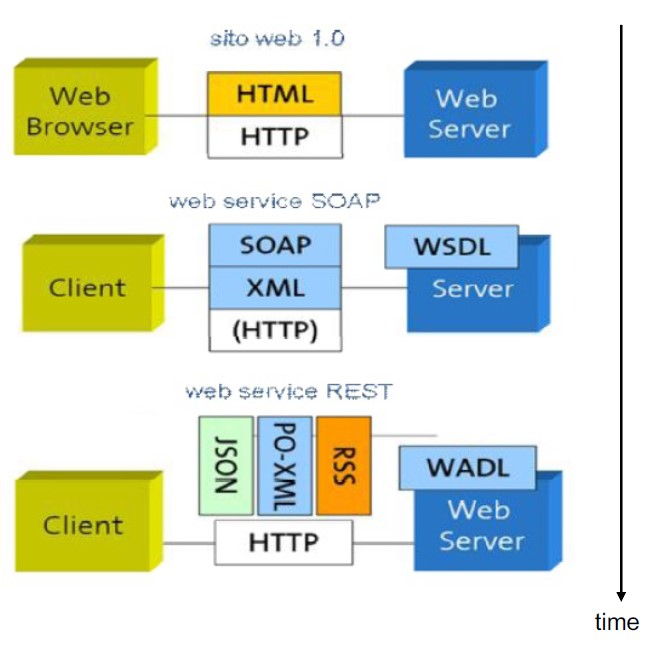
\includegraphics[width=0.5\textwidth]{img/REST1.jpg}
\end{center}
Come abbiamo visto ieri, per la struttura al centro dell'immagine, SOAP è la struttura dei messaggi, XML la tecnologia abilitante (giusto?) e HTTP il protocollo di scrittura. Questo ci porta ai servizi del server WSDL.

\section{REST vs SOAP}
\begin{center}
    \begin{tabular}{ |c|c|c| } 
        \hline
         & \textbf{REST} & \textbf{SOAP} \\ 
        \textbf{Transport Protocol} & HTTP & diversi protocolli (e.g., HTTP, TCP, SMTP) \\ 
        cell7 & cell8 & cell9 \\ 
        \hline
    \end{tabular}
\end{center}





\section{Composition = Establishing a Common Model}
I sistemi distribuiti per funzionare devono basarsi su modelli comuni,
\begin{itemize}
    \item WSDL/i sistemi SOAP SOA si devono accordare su API che comunicano tramite formati di messaggi comuni 
    \item Very well defined but resulted overcomplex
\end{itemize}
REST is built around the idea of simplifying the agreement
1. \textbf{nouns} are required to name the resources that can be talked about (exchanged, deleted, created)
2. \textbf{verbs} are the operations that can be applied to named resources (get per ottenere una risorsa, post per non lo so, etc\dots)
3. \textbf{content types} (e.g., application/json) define which information representations are available, rappresentazione che vogliamo dare ad una risorsa

\subsubsection{Es. piano registrazione esami studenti}
\textbf{Managing the university curriculum}
§ Same data -> Different representations: administrative - didactics
§ Machine-oriented ( XML/JSON) - human-oriented (HTML) representations
§ Links (URIs) define possible resource manipulation actions. Examples of endpoints:
→ GET unimib.it/{matricola}: returns information about the student and list of available actions:
§ unimib.it/{matricola}/cambiaPianoStudio
§ unimib.it/{matricola}/pianoStudio
§ unimib.it/{matricola}/administration
→ unimib.it/{matricola}/pianoStudio:
§ GET list of exams the student is registered for,
§ POST register for an exam,
§ PUT modify exam registration,
§ DELETE exam registration
→ unimib.it/{matricola}/pianoStudio/{code}:
§ GET information about the exam the student is registered for

\section{Principi REST}
\textbf{REST} = \textbf{RE}presentational \textbf{S}tate \textbf{T}ransfer
REST is an \textbf{architectural style} for distributed systems
\\Resources are defined by URIs (che di solito hanno questa struttura: /baseURL/resourceType/{id})
\\Resources are manipulated through their representations. There can be multiple representations for a resource (e.g., XML, JSON, HTML)
\\La communicazione avviene per messaggi, tutti semplici (stateless, privi di stato), autodescrittivi (devono contenere una descrizione dei dati); l'unico modo per interargirci è per richiesta-risposta. Una conseguenza è il poter usare solo get e post (ho capito bene?)
\\Application state is driven by resource manipulations.
\\Hypermedia is the way to control application behavior (altri link perché il Client possa scoprire da solo posibili manipolazioni effettuabili su tale risorsa).
\\N.B.: REST principles nicely fit the Web architectural components: URI and HTTP.

\section{Representational State Transfer}
Key information (data) abstraction: the resource
§ A resource is any information that can be named: documents, images, services, people, collections, etc.
§ Resources have/are state
§ Resources may change over time
§ Resources usually change with the interaction with the client
§ Resources have identifiers (constraint) che sono dinamici (unimib.it/{matricola}/pianoStudio)
§ {matricola} is called path parameter
§ A resource is anything important enough to be referenced
§ Resources expose a uniform interface (constraint)
§ GET, POST, PUT, DELETE + Identifiers in the URI
§ System architecture simplified; visibility improved.
§ Encourages independent evolvability of implementations.
On request, a service may transfer a representation of the resource to a client
§ Requires a client-server architecture (constraint)
§ E.g., list of the exams registered for a certain student id
§ A client may transfer a modified representation of a resource
§ Manipulation of resources through representations (constraint) - no action invocation
§ E.g., a student can alter the list of exams by adding a new registration to the list
§ Representations returned from the server should link to additional representations/actions. Clients may
follow a proposed link and assume a new state
§ Hypermedia as the engine of application state (constraint)
§ E.g., beside the list of registered exams, a link to add or delete a registration can be present
Stateless interactions (constraint)
§ Each request from client to server must contain all the information necessary to understand the request, and \underline{cannot
take advantage of any stored context on the server}
§ Statelessness necessitates \textbf{self-descriptive messages} (constraint)
§ Standard media types (example, application/json)
§ Meta-data and control-data
§ Uniform interface + Stateless + Self-descriptive = Cacheable (può essere mantenuta in una cache, che in un'interazione web è uno spazio di memoria dedicato alla comunicazione Client-Server, questo funziona solo se il messaggio è completo ovvero self-descriptive) (constraint)
§ Cacheability necessitates a layered-system (constraint)
§ A cache layer is necessary
§ In the cache is stored the latest representation of a resource
§ A cache is invalidated upon resource state alteration (PUT, DELETE)

\section{Caching}
§ Caching reduces latency and network traffic
§ Only (non-SSL) GETs are cached – not POSTs etc.
§ Two kinds of caches
§ Client-side (for instance in the browser)
§ Proxy/server
§ Large SOAs use a caching proxy server (memcache, et similia)
§ You may be using it and not even know it
§ Remember, there can be caches all along the way

\subsection{Local caching}
Nell'immagine mostrata vediamo il server ricevere l'informazione: riceve come dato 200, e il cache-control mi dice "ok, nei prossimi 120 secondi (max-age = 120) l'informazione non dovrebbe cambiare, tieni l'informazione in cache".
\begin{center}
    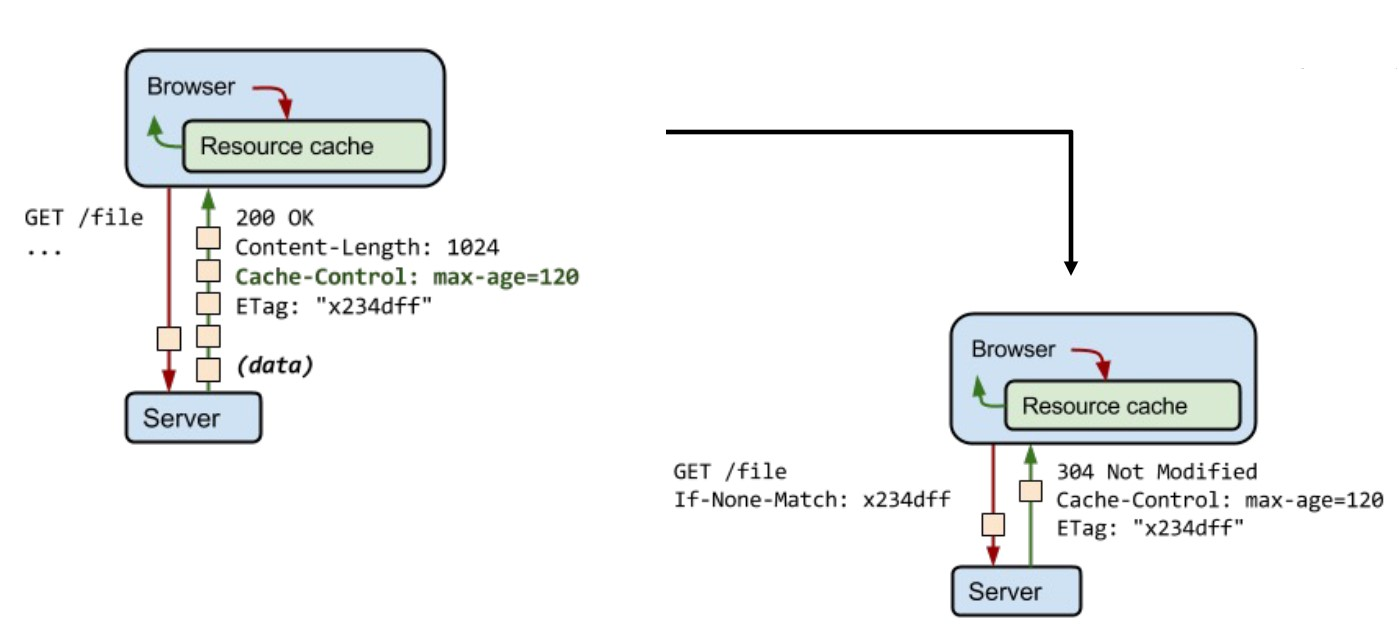
\includegraphics[width=0.5\textwidth]{img/REST2.jpg}
\end{center}

\section{Alcune osservazioni}
REST is all about simplicity
§ Caching improves response time and reduces server load
§ Statelessness and less communication enables easier load balancing between servers
§ Less specialized software because the underlying technologies are well known and simple
§ Identification is done using standard mechanisms, no additional names necessary
REST is (based on) standard(s)
§ REST principles emphasizes the correct and complete use of the HTTP protocol to publish services on the Web.
§ REST over HTTP provides a lightweight and layered mechanisms for data and service integration.
§ REST with HTTP protocol provides a distributed, hypermedia-driven application platform.

\section{Using HTTP to build REST Applications}
\begin{center}
    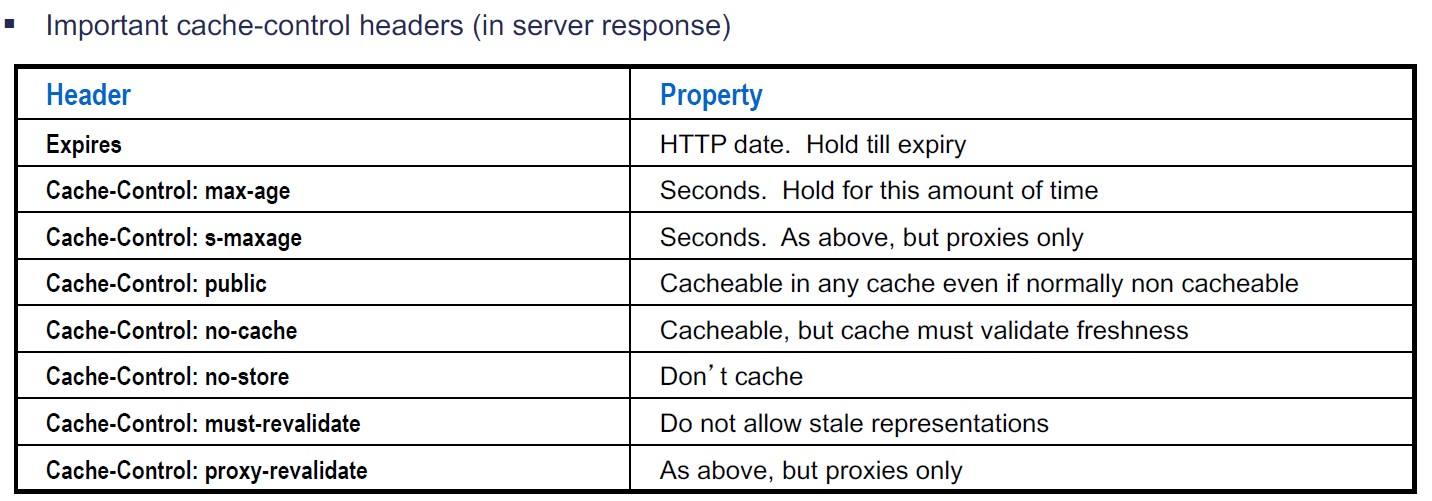
\includegraphics[width=0.5\textwidth]{img/REST3.jpg}
\end{center}
The REST Recipe:
§ Find all the nouns
§ Define the formats
§ Pick the operations
§ Highlight exceptional status codes
Find all the nouns: saper scegliere i nomi a tutte le risorse è la cosa più difficile da fare in un REST.
§ Everything in a RESTful system is a resource – a noun
§ If you find yourself creating verbs, noun-ify them (ApproveExpense à ExpenseApprovals)
§ Every resource has a URI. Ideally just one (but don't sweat it)
§ URIs should be descriptive
§ http://example.com/expenses/pending
§ Spend some time here, but don't agonize over the perfect URI
§ URIs should be opaque \verb|(https://www.w3.org/DesignIssues/Axioms.html#opaque)|
§ automated (non-human) clients should not infer meta-data from a URI
§ URIs should be cool - persistent (http://www.w3.org/Provider/Style/URI)
§ Cool URIs don't change (simplicity, stability, manageability)
§ Foundation requirement of the semantic web
Avere una gerarchia d'accesso alle risorse obbliga il Cliente a fare che?
\\Capita che la versione dell'API di un servizio evolva: di solito si crea una versione nuova mantenendo attiva quella precedente.
\\Find all the nouns
§ Use path variables to encode hierarchy
§ /expenses/pending/123 (/expenses/pending/{id})
§ Use other punctuation to avoid implying hierarchy
/expenses/Q107;Q307
/expenses/lacey,peter
§ Use query variables to imply filtering conditions
\begin{verbatim}
    /search?approved=false
\end{verbatim}
§ You won't need query variables as much as you think
\begin{verbatim}
    /expenses?start=20070101&end=20071231
\end{verbatim}
should be
/expenses/20070101-20071231
§ Caches tend to (wrongly) ignore URIs with query variables
§ URI space is infinite (but URI length is not ~ 4K)
§ Don't leak platform information
/expenses.php/123

\subsection{Defining the formats}
Neither HTTP nor REST mandate a single representation for data
§ A resource may have multiple representations
XML, JSON, binary (e.g., jpeg), name/value pairs
§ Schema languages are not required (if even possible)
§ Avoid creating custom representations: use well-known media types (IANA registered MIME types)
§ Makes content more accessible
§ Part of the self-descriptive messaging constraint
§ Incoming representations should be the same as outgoing representations
§ A client should be able to GET, modify, and PUT a document
§ Server should discard any extraneous data

\subsection{Pick the operations}
§ Pick the operations which can be applied to resources
§ HTTP has a constrained user interface (set of verbs/operations/methods)
§ For most applications, HTTP's basic methods are sufficient
§ GET : Fetching a resource (there must be no side-effects)
§ POST : Adds to a new resource on the server
§ PUT : Transfers a resource to a server (overwriting if there already is one) - Update
§ DELETE : Discards a resource
§ More methods are available
§ HEAD like GET but without body
§ OPTIONS (not widely supported)
§ Patch applies a partial update to the resource ( you are only required to send the data that you want to update)
§ TRACE (not significant)
§ CONNECT (not significant)
§ All our resources will support GET

\section{Operazioni HTTP}
\begin{center}
    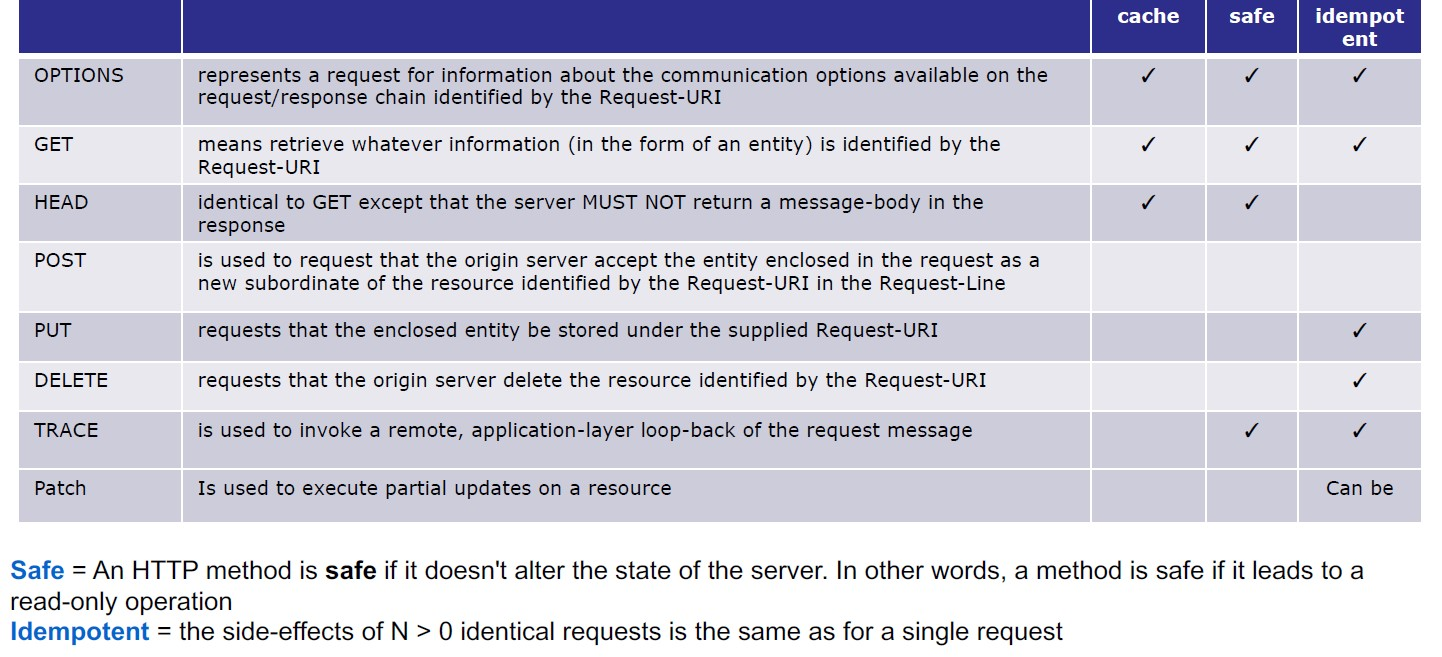
\includegraphics[width=0.5\textwidth]{img/REST4.jpg}
\end{center}
Perché GET è idempotente? Me lo sono perso.
Perché POST è idempotente? Perché ogni volta che lo eseguo mi si crea una nuova risorsa con il proprio identificativo.

\section{REST come implementazione CRUD}
\begin{center}
    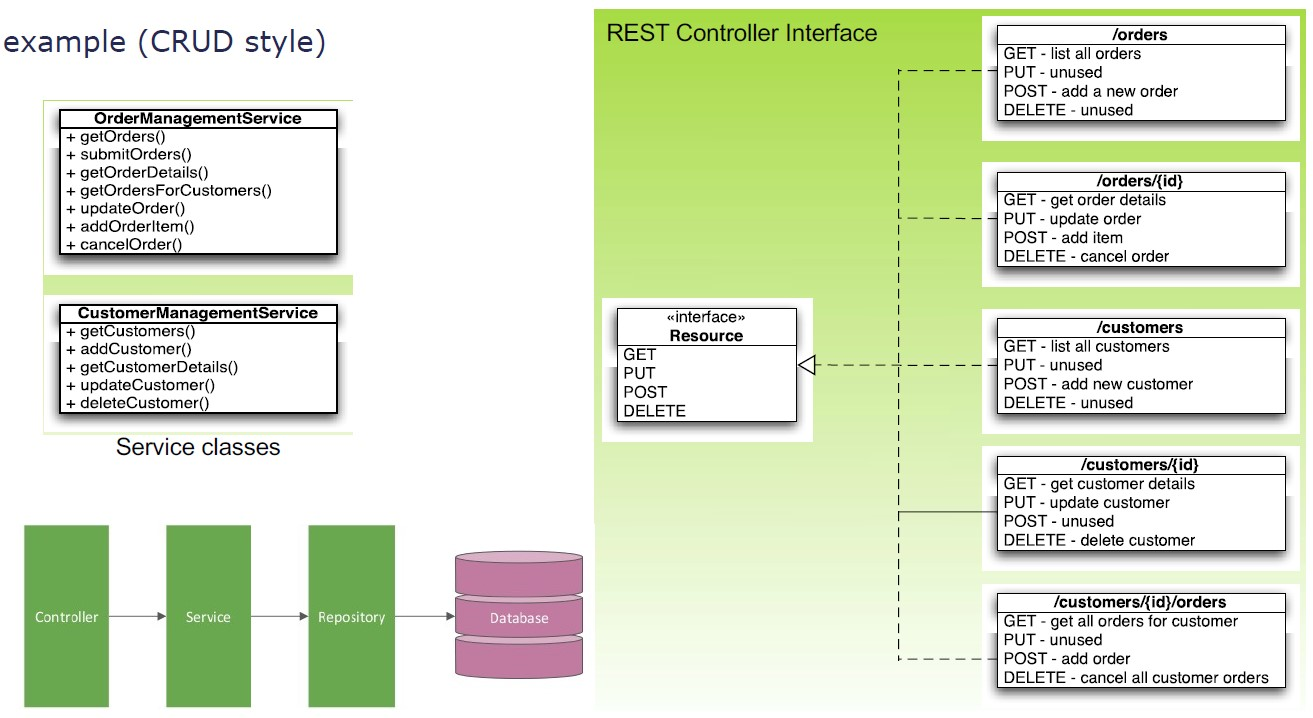
\includegraphics[width=0.5\textwidth]{img/REST5.jpg}
\end{center}

\subsection{Response Status Code}
The response status code is generated by the server to indicate the outcome of a request.
\\The status code is a 3-digit number:
\begin{itemize}
    \item 1xx (Informational): Request received; server is continuing the process.
    \item 2xx (Success): Request received, understood, accepted and serviced.
    \item 3xx (Redirection): Further action must be taken in order to complete the request.
    \item 4xx (Client Error): The request contains bad syntax or cannot be understood.
    \item 5xx (Server Error): The server failed to fulfill an apparently valid request.
\end{itemize}
Proper identification of status codes associated with a request is a crucial decision in REST development.

\section{PUT vs. POST}
When creating new resources
§ Use POST if the server chooses the URI (the id)
§ Use PUT if the client chooses the URI (the id)
§ POST can be used as "Process this"
§ POST does "something" and returns "something"
§ Usually masking a Remote Procedure Call (RPC) (overloaded POST) - function invocation
§ Don't use it casually
§ "Process this" POST sometimes valuable:
§ Resource factories
§ Sometimes you just want a verb
§ If you find yourself creating resources that can't be retrieved with GET, reexamine your design
\begin{verbatim}
    http://expense.example.com/pay_expense
\end{verbatim}
§ But don't sweat it, if it gets you out of a design jam

Ho saltato alcune slides

\section*{Hypermedia control}
HATEOAS: Hypermedia As The Engine Of Application State
§ Application state manipulation = the current state manipulated by the client
§ Hypermedia = links and forms
§ Following a link can be seen as an application state transition
§ Server provides a new representation; client assumes that state
§ The server “guides” the client to new states by providing links inside resource representations
§ All representations should contain links
§ No links, no Web  
sono tre simplified